\documentclass{article}
\usepackage{graphicx} % Required for inserting images
\usepackage[italian]{babel}
\usepackage{amsmath}
\usepackage[hidelinks]{hyperref}
\usepackage{amssymb}
\usepackage{xcolor}

\newcommand{\defeq}{\overset{\mathrm{def}}{=\joinrel=}}

\newcommand{\ubar}[1]{\text{\b{$#1$}}}

\newtheorem{theorem}{Teorema}

\title{Calcolo integrale}
\author{Leonardo Ganzaroli}
\date{}

\begin{document}

\maketitle

\addcontentsline{toc}{section}{\protect\numberline{}Introduzione}

\tableofcontents

\newpage

\hypersetup{allcolors=black}

\section*{Introduzione}

Questi appunti del corso \textit{Calcolo integrale} sono stati creati durante la laurea Triennale di informatica all'università "La Sapienza".\newline

\noindent \textbf{N.B. Questo corso è il naturale proseguimento di \textit{Calcolo differenziale}, quindi molte cose saranno date per scontate}.

\newpage

\section{Serie numeriche}

\noindent\textbf{Definizione} Una successione di elementi è un elenco ordinato dei valori assunti dalla funzione $a:S\subseteq\mathbf{N}\rightarrow A:k\rightarrow a_k$, essa associa dei valori ad un sottoinsieme dei numeri naturali presenti in $A$ che solitamente $\subset\mathbf{R}\ \vee \subset\mathbf{C}$.\newline

\noindent\rule{\textwidth}{0.5pt}

\noindent Alcune successioni:
\begin{itemize}
    \item $3k=3,6,9,12,\ldots$
    \item $k^2=1,4,9,16,\ldots$
    \item $k+1=2,3,4,\ldots$
\end{itemize}

\noindent\rule{\textwidth}{0.5pt}\newline

\noindent\textbf{Definizione} Si definisce $S_n$ come la sommatoria dei primi $n$ numeri di una successione.\newline

\noindent\textbf{Definizione} Si definisce serie numerica il limite per $n\rightarrow+\infty$ di $S_n$:

$$\lim_{n\rightarrow+\infty}\sum_{k=1}^{n}a_k$$\newline

\noindent \textbf{Da qui in poi si assuma che $k\in\mathbf{N^+}$.}\newline

\noindent\textbf{Definizione} Se una serie numerica equivale ad un valore finito $l$ allora è convergente ad $l$.\newline

\noindent\textbf{Definizione} Se una serie numerica equivale a $\pm\infty$ allora è divergente.\newline

\begin{theorem}[Serie a termini di segno costante]
    $\ $\newline
    \begin{itemize}
        \item $\forall k\in\mathbf{N^+}\ a_k\geq0\Rightarrow \sum_{k=0}^{+\infty}a_k$ converge ad un valore positivo o diverge a $+\infty$

        \item $\forall k\in\mathbf{N^+}\ a_k\leq0\Rightarrow \sum_{k=0}^{+\infty}a_k$ converge ad un valore negativo o diverge a $-\infty$\newline
        
    \end{itemize}
\end{theorem}

\begin{theorem}[Condizione necessaria per la convergenza]$\ $\newline
    $$\sum_{k=0}^{+\infty}a_k \text{ converge }\Rightarrow \lim_{n\rightarrow+\infty}a_n=0$$\newline
\end{theorem}

\subsection{Criteri}

\begin{theorem}[Criterio del confronto diretto]$\ $\newline
    Date 2 successioni $a_n,b_n\ |\ \exists N\in\mathbf{N}\ |\ \forall n\geq N\ \ 0\leq a_n\leq b_n$ si ha:
    $$\sum_{k=0}^{+\infty}b_k \text{ converge }\Rightarrow\sum_{k=0}^{+\infty}a_k\text{ converge }$$
\end{theorem}

\vspace{8pt}

\begin{theorem}[Criterio del confronto asintotico]$\ $\newline
    Date 2 successioni $a_n,b_n\ |\ \lim_{n\rightarrow+\infty}\frac{a_n}{b_n}=\delta$ con $0<\delta<+\infty$ si ha:
    $$\sum_{k=0}^{+\infty}a_k \text{ converge }\iff\sum_{k=0}^{+\infty}b_k\text{ converge }$$
\end{theorem}

\vspace{8pt}

\begin{theorem}[Criterio del rapporto]$\ $\newline
    Data la successione a termini positivi $a_n\ |\ \lim_{n\rightarrow+\infty}\frac{a_{n+1}}{a_n}=\delta$ con $0\leq\delta<+\infty$ si ha:
    \begin{itemize}
        \item $\delta<1$ converge
        \item $\delta>1$ diverge
    \end{itemize}
\end{theorem}

\vspace{8pt}

\begin{theorem}[Criterio della radice]$\ $\newline
    Data la successione a termini positivi $a_n\ |\ \lim_{n\rightarrow+\infty}\sqrt[n]{a_n}=\delta$ con $0\leq\delta<+\infty$ si ha:
    \begin{itemize}
        \item $\delta<1$ converge
        \item $\delta>1$ diverge
    \end{itemize}
\end{theorem}

\vspace{8pt}

\begin{theorem}[Criterio di Leibniz]$\ $\newline
    Data la successione a segno alterno $a_n=(-1)^k*b_k$, se:
    \begin{itemize}
        \item $b_k$ ha termini di segno non negativo
        \item $\forall k\in\mathbf{N^+}\ \ b_{k+1}\leq b_k$
        \item $\lim_{n\rightarrow+\infty}b_n=0$
    \end{itemize}

    \noindent Allora $\sum_{k=0}^{+\infty}a_k$ converge.
    
\end{theorem}

\vspace{8pt}

\begin{theorem}[Criterio di convergenza assoluta]$\ $\newline

    $$\sum_{k=0}^{\infty}|a_k| \text{ converge }\Rightarrow\sum_{k=0}^{\infty}a_k\text{ converge }$$

\end{theorem}

\subsection{Serie di potenze}

\textbf{Definizione} Una serie di potenze di centro $x_0$ associata ad una successione è:

$$\sum_{k=0}^{\infty}a_k*(x-x_0)^k$$\newline

\noindent\textbf{Definizione} Un insieme di convergenza è l'intervallo $X\subseteq\mathbf{R}$ per cui:

$$\forall\ x\in X\ \ \exists l\in\mathbf{R}\ |\ l=\sum_{k=0}^{\infty}a_k*(x-x_0)^k$$\newline

\noindent\textbf{Definizione} Il raggio di convergenza di una serie di potenze è:

$$p=sup\{x\geq0\ |\ \sum_{k=0}^{\infty}a_k*(p-x_0)^k\text{ converge}\}$$\newline

\begin{theorem}[Calcolo del raggio di convergenza]

$$p=\lim_{k\rightarrow+\infty}\frac{1}{\sqrt[n]{|a_n|}}$$\newline
    
\end{theorem}

\noindent\textbf{Definizione} La serie di Taylor di $f$ di centro $x_0$ è il polinomio di Taylor di ordine $+\infty$.\newline

\newpage

\section{Integrali}

Per poter trovare l'area sottostante ad una funzione in un certo intervallo è possibile scomporre quell'area in una serie di rettangoli e sommarne le aree, per evitare approssimazioni il metodo migliore è usare la più grande quantità di rettangoli possibile con la stessa larghezza.\newline

\noindent Ci sono 2 possibilità per ricoprire l'area:
\begin{enumerate}
    \item \textcolor{blue}{Rettangoli maggiori}, la somma delle loro aree si indica con $\bar{S_n}$
    \item \textcolor{red}{Rettangoli minori}, la somma delle loro aree si indica con $\ubar{S_n}$
\end{enumerate}

\begin{figure}[ht]
    \centering
    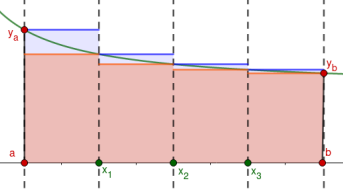
\includegraphics[width=0.5\linewidth]{rett.png}
    \label{fig:rett}
\end{figure}

\noindent Considerando un numero di rettangoli infiniti si ottiene:

$$\lim_{n\rightarrow+\infty}\bar{S_n}=\bar{S}=\text{Area}=\ubar{S}=\lim_{n\rightarrow+\infty}\ubar{S_n}$$\newline

\noindent\textbf{Definizione} Data una funzione $f:[a,b]\subset\mathbf{R}\rightarrow\mathbf{R}$. $f$ è integrabile secondo Riemann se è vera l'equazione vista sopra, si definisce integrale di $f$ nell'intervallo $[a,b]$:

$$\int_a^bf(x)\ dx$$

\noindent Inoltre per risultare integrabile la funzione deve essere continua e limitata.\newline



\noindent In particolare risulta:
\begin{itemize}
    \item limite di $\bar{S_n}$

        $$\lim_{n\rightarrow+\infty}\frac{b-a}{2^n}*\sum_{k=0}^{2^n-1}max_{[x_k,x_{k+1}]}f(x)$$

    \item limite di $\ubar{S_n}$

        $$\lim_{n\rightarrow+\infty}\frac{b-a}{2^n}*\sum_{k=0}^{2^n-1}min_{[x_k,x_{k+1}]}f(x)$$
    
\end{itemize}

\subsection{Proprietà}

\begin{theorem}[Linearità]
    Date $f,g$ integrabili nell'intervallo $[a,b]$. La funzione $h(x)=\alpha f(x)+\beta g(x)$ è integrabile in $[a,b]$ ed il suo integrale equivale alla somma dei 2 integrali:

$$\alpha\int_a^bf(x)\ dx+\beta\int_a^bg(x)\ dx$$\newline
    
\end{theorem}

\begin{theorem}[Additività]
    Se $f$ è integrabile in $[a,c]=[a,b]\cup[b,c]$ allora l'integrale di $[a,c]$ è la somma degli integrali dei sottointervalli.\newline
    
\end{theorem}

\begin{theorem}[Differenza]
    Se $f$ è integrabile in $[a,b]$ allora l'integrale in $[c,b]$ con $c\in[a,b]$ è la differenza tra l'integrale di $[a,b]$ e quello di $[a,c]$.\newline
    
\end{theorem}

\begin{theorem}[Inversione dell'intervallo]
    Se $f$ è integrabile in $[a,b]$ e $a<b$ vale:
    
    $$\int_a^bf(x)\ dx=-\int_b^af(x)\ dx$$\newline
    
\end{theorem}

\subsection{Teorema fondamentale del Calcolo integrale}

\begin{theorem}[Teorema fondamentale del Calcolo integrale]$\ $\newline
    Data $f:[a,b]\rightarrow\mathbf{R}$ continua, limitata e integrabile:

    $$\left(F(t)=\int_a^tf(x)\ dx\text{ con $a\leq t\leq b$ }\right)\Rightarrow\forall t\in[a,b]\ \  F'(t)=f(t)$$

\noindent In breve $F$ è l'antiderivata di $f$.\newline
    
\end{theorem}

\noindent\textbf{Definizione} Una funzione $G(x)\ |\ G'(x)=f(x)$ è detta primitiva di $f(x)$, inoltre tutte le sue primitive hanno forma $F(x)+c\ \ \forall c\in\mathbf{R}$.\newline

\newpage

\noindent\textbf{Definizione} Si definiscono 2 tipi di integrali:
    \begin{itemize}
        \item \textbf{Definito}

            $$\int_a^bf(x)=F(x)\ |_a^b=F(b)-F(a)$$
        
        \item \textbf{Indefinito}

            $$\int f(x)=F(x)+c$$\newline
        
    \end{itemize}

\noindent\rule{\textwidth}{0.5pt}

\noindent Calcolo $\int_2^8x^2+5x\ dx$:
    \begin{itemize}
        \item L'antiderivata è $\frac{x^3}{3}+\frac{5x^2}{2}$
        \item L'integrale sarà quindi $\frac{8^3}{3}+\frac{5*8^2}{2}-\frac{2^3}{3}+\frac{5*2^2}{2}=318$
    \end{itemize}

\noindent\rule{\textwidth}{0.5pt}\newline

\begin{theorem}[Pari e dispari]$\ $\newline
    Dato un integrale su $[0,t]$:

    $$f(x)\text{ è pari }\Rightarrow F(t)\text{ è dispari\ \ \ \  (o viceversa)}$$\newline

\end{theorem}

\begin{theorem}[Pari e dispari 2]$\ $\newline
    Dato un integrale su $[-t,t]$:

    \begin{itemize}
        \item $f(x)$ dispari

        $$\int_{-t}^tf(x)=0$$

        \item $f(x)$ pari

        $$\int_{-t}^tf(x)=2\int_0^tf(x)$$\newline
        
    \end{itemize}

\end{theorem}

\subsection{Integrali impropri}

\textbf{Definizione} Un integrale improprio è il limite di un integrale definito al tendere di almeno un estremo di integrazione ad un numero reale oppure all'infinito, quel numero reale può rappresentare un punto di discontinuità.\newline 

\noindent Possono avere 4 possibili forme (il limite si omette solitamente):
\begin{enumerate}
    \item $\int_a^\infty f(x)\ dx$
    \item $\int_{-\infty}^b f(x)\ dx$
    \item $\int_{-\infty}^\infty f(x)\ dx$
    \item $\int_a^b f(x)\ dx$ con $f(x)$ indefinita o discontinua da qualche parte in $[a,b]$\newline
\end{enumerate}

\noindent\textbf{Definizione} Data $f$ divergente in un certo punto in $[a,b]$.\newline

$f$ si dice integrabile in senso improprio su $[a,b]$ se:
\begin{itemize}

    \item Il punto in cui diverge è $a$ e $\lim_{\epsilon\rightarrow0^+}\int_{a+\epsilon}^bf(x)\ dx=l$

    \item Il punto in cui diverge è $b$ e $\lim_{\epsilon\rightarrow0^+}\int_a^{b-\epsilon}f(x)\ dx=l$

    \item Diverge sia in $a$ che in $b$ e $\lim_{\epsilon\rightarrow0^+,\delta\rightarrow0^+}\int_{a+\epsilon}^{b-\delta}f(x)\ dx=l$\newline
    
\end{itemize}

\noindent Similmente se l'intervallo presenta almeno un infinito:
\begin{itemize}

    \item $[a,+\infty)$ e $\lim_{z\rightarrow+\infty}\int_{a}^zf(x)\ dx=l$

    \item $(-\infty,b]$ e $\lim_{z\rightarrow-\infty}\int_{z}^bf(x)\ dx=l$

    \item $(-\infty,+\infty)$ e $\int_{-\infty}^cf(x)\ dx+\int_c^{+\infty}f(x)\ dx=l\ \text{ per qualche $c$}$\newline

\end{itemize}

\newpage

\subsubsection{Convergenza}

Si considerino tutte le funzioni prese in considerazione in questa sezione aventi $x_0$ come punto di discontinuità.\newline

\begin{theorem}[Criterio del confronto asintotico]$\ $\newline
    $$\text{Se }\left(\lim_{x\rightarrow x_0}\frac{f(x)}{g(x)}=l\Rightarrow\int_a^{x_0}f(x)\ dx\approx\int_a^{x_0}g(x)\ dx\right)$$
    $$\text{allora\  (l'integrale di } g(x)\text{ converge}\iff\text{l'integrale di } f(x) \text{ converge)}$$\newline
\end{theorem}

\begin{theorem}[Criterio del confronto diretto]
    $$\text{Se }\left(0\leq\int_a^{x_0}f(x)\ dx\leq\int_a^{x_0}g(x)\ dx\right)$$
    $$\text{allora\  (l'integrale di } g(x)\text{ converge}\Rightarrow\text{l'integrale di } f(x) \text{ converge)}$$\newline
\end{theorem}

\begin{theorem}[Criterio di convergenza assoluta]
    $$\int_a^{x_0}|f(x)|\ dx<+\infty\Rightarrow\int_a^{x_0}f(x)\ dx<+\infty$$
\end{theorem}

\newpage

\section{Equazioni differenziali}

\textbf{Definizione} Un'equazione differenziale è un'equazione che lega una funzione incognita alle sue derivate.

\subsection{EDO}

\textbf{Definizione} Un'equazione differenziale ordinaria coinvolge una funzione di una variabile e le sue derivate di ordine qualsiasi.\newline

\noindent\textbf{Definizione} L'ordine di una EDO è il più alto ordine tra le derivate che contiene.

\vspace{5pt}

\noindent\rule{\textwidth}{0.5pt}

\noindent Per esempio l'accelerazione istantanea di un corpo è data dalla derivata della velocità istantanea che a sua volta è la derivata della funzione dello spostamento del corpo:

$$a(t)=v'(t)=s''(t)$$\newline

\noindent Ipotizzando che l'accelerazione abbia valore $a\frac{m}{s^2}$ riscrivo:

$$a(t)=s''(t)=a\frac{m}{s^2}$$\newline

\noindent Posso ricavare la funzione integrando 2 volte $s''(t)$:

\begin{equation}
    \nonumber
    \begin{split}
        \int\int s''(t)\ dt\ dt&=\int\int a\ dt\ dt\\
        &=\int(at+c_1)\ dt\\
        &=\frac{at^2}{2}+c_1t+c_2
    \end{split}
\end{equation}

\noindent\rule{\textwidth}{0.5pt}\newline

\noindent\textbf{Definizione} Il problema di Cauchy consiste nel trovare la soluzione di un'equazione differenziale di ordine $n:f(x,y(x),y''(x),\ldots,y^n(x))=0$ tale che soddisfi le condizioni iniziali:

\begin{equation}
    \nonumber
    \begin{split}
        y(a)&=y_0\\
        y'(a)&=y_1\\
        y''(a)&=y_2\\
        \ldots\\
        y^{n-1}(a)&=y_{n-1}
    \end{split}
\end{equation}

\subsubsection{EDO lineari}

\textbf{Definizione} Una EDO è definita lineare se:
\begin{enumerate}
    \item è lineare ($y(t)$ e $y'(t)$ hanno grado 0 o 1)
    \item è omogenea (non ci sono termini costanti aggiuntivi indipendenti da $y(t)$)\newline
\end{enumerate}

\noindent In questo caso se ho un'equazione della forma:

\[
\begin{cases}
    y'(t)=a(t)y(t)+b(t)\\
    y(t_0)=y_0
\end{cases}
\]\newline

\noindent posso riscrivere il problema di Cauchy come:

$$y(t)=\mathbf{e}^{A(t)}\left[y_0+\int_{t_0}^tb(t)\mathbf{e}^{-A(t)}\ dt\right]$$

\end{document}
